\paragraph{}Ta projektna naloga se osredotoča na strukturo in razvoj zadnje različice aplikacije, verzije 3.0. Ta je objavljena na spletni trgovini Google Play na naslovu \url{https://play.google.com/store/apps/details?id=com.zigapk.gimvic.suplence}. Aplikacija je odprtokodna, njena izvorna koda pa je dostopna na spletnem portalu Github na naslovu \url{https://github.com/GimVic-app/gimvic-android/}.

\subsection{Pridobivanje podatkov}
\paragraph{}Aplikacija za svoje delovanje potrebuje podatke o:
\begin{itemize}
  \setlength\itemsep{0em}
  \item nadomeščanjih,
  \item urniku in
  \item jedilniku.
\end{itemize}

\paragraph{}Te se nahajajo na več različnih strežnikih v zelo različnih oblikah. Podatki o nadomeščanjih se pridobijo s spletne storitve elektronske redovalnice Gimnazije Vič v JSON\cite{json-wiki} (ang. \textit{JavaScript Object Notation}). Podatki o urniku za vse razrede in učitelje so na voljo na naslovu \url{http://old.gimvic.org/urnik/data.js}\cite{rin} v obliki izvorne kode JavaScript, ki generira tabelo. Sistem za pridobivanje podatkov o jedilniku pa je bilo treba še razviti.

\paragraph{}Posamezne jedilnike (več vrst malic in kosila) sestavlja na svojem računalniku organizatorica šolske prehrane ga. Eva Jelen v programu Excel. Da bi te podatke lahko dostavili in obdelali na strežniku, sem pripravil vtičnik za Excel, ki je dostopen na povezavi \url{https://github.com/GimVic-app/menu-uploader}. Ta je nameščen na njenem računalniku, tako da so lahko podatki o jedilnikih z enim klikom posodobljeni na spletnem strežniku.

\paragraph{}Da se izognemo nepotrebnemu in zahtevnemu obdelovanju podatkov na telefonu, je koncept delovanja zasnovan na sistemu strežnik - odjemalec. Na strežniku tečeta dva programa, ki mobilni aplikaciji zagotavljata željene podatke. To sta:
\begin{itemize}
  \setlength\itemsep{0em}
  \item posodobljevalnik podatkov in
  \item glavna strežniška aplikacija.
\end{itemize}

\paragraph{}Vsi zbrani podatki se v tej različici zberejo na strežniku in obdelajo ter shranijo v relacijsko podatkovno bazo MySQL\cite{mysql-wiki}. Temu je namenjen program Posodobljevalnik podatkov, dostopen na naslovu \url{https://github.com/GimVic-app/data-updater}. Podatki o urniku in nadomeščanjih se posodabljajo ob nastavljenih časovnih intervalih, podatki o jedilniku pa takoj, ko so posodobitve na voljo.

\paragraph{}Da lahko mobilna aplikacija  do podatkov v bazi dostopa prek interneta, je bilo potrebno napisati še glavno strežniško aplikacijo, ki prepozna uporabnikove nastavitve in na zahtevo mobilni aplikaciji postreže z željenimi podatki. Glavna strežniška aplikacija je napisana v programskem jeziku Go, njena izvorna koda pa je dostopna na naslovu \url{https://github.com/GimVic-app/server}.

\paragraph{}Mobilna aplikacija lahko tako s preprosto poizvedbo na strežnik dobi vse podatke v obliki JSON\cite{json-wiki}. Uporabnikove nastavitve aplikacija definira kar s parametri\cite{query-wiki} v URL naslovu. Podatki, ki jih strežnik vrne, vsebujejo seznam dni in za vsak dan natančno opisan urnik, morebitna nadomeščanja ter jedilnik.

\paragraph{}Celotna infrastruktura za pridobivanje, obdelavo in streženje podatkov je postavljena na strežniškem operacijskem sistemu Debian\cite{debian-wiki} različice 8 (\textit{Jessie}). Ta teče na virtualnem strežniku, ki ga je za potrebe aplikacije GimVic prijazno zagotovil Zavod 404 in je dostopen na spletnem naslovu \url{http://gimvicapp.404.si/}.

\subsection{Struktura aplikacije}
\paragraph{}Aplikacija je sestavljena iz več aktivnosti (ang. \textit{activities}). Najpomembnejše so:
\begin{itemize}
  \setlength\itemsep{0em}
  \item upravitelj podatkov,
  \item prikazovalnik podatkov,
  \item aktivnost za upravljanje z nastavitvami,
  \item aktivnost za izbiranje filtrov.
\end{itemize}

\subsubsection{Upravitelj podatkov}
\paragraph{}Upravitelj podatkov podaja informacije prikazovalniku podatkov. Te pridobiva v rednih intervalih s strežnika. V poizvedbah strežniku poda tudi uporabnikove nastavitve. Če glavna aktivnost potrebuje podatke, internetne povezave pa ni, upravitelj podatkov poda zadnje veljavne podatke, ki so shranjeni na napravi skupaj z datumom in časom zadnje posodobitve. Slednje je namenjeno uporabniku kot indikator ažurnosti podatkov.

\subsubsection{Prikazovalnik podatkov}
\paragraph{}Prikazovalnik podatkov (slika \ref{fig:main_activity}) uporabniku v obliki pregledne tabele izpiše njegov urnik ter jedilnik. Omogoča preprosto pomikanje med posameznimi dnevi v tednu ter vsebuje tudi povezavo do nastavitev. Podatke za prikazovanje dobi od upravitelja podatkov.

\subsubsection{Nastavitve}
\paragraph{}Nastavitve (slika \ref{fig:settings_activity}) omogočajo uporabniku nastavljanje vrste malice, kosila ter vklop oz. izklop prikazovanja nadomeščanj. Vsebujejo tudi gumb, ki uporabnika popelje na stran za izbiro razredov ter osnovne podatke o različici in avtorju aplikacije.

\subsubsection{Izbira filtrov}
\paragraph{}Aktivnost za izbiro filtrov (slika \ref{fig:filters_activity}) dijakom omogoča, da izberejo svoj razred in morebitne izbirne predmete, profesorjem pa, da izberejo svoj urnik. Po dogovoru z ravnateljico mag. Alenko Krapež je izbira razreda omejena na 5 sprememb, izbira profesorja pa zaščitena z univerzalnim profesorskim geslom.

% images
\begin{figure}[!htb]
\minipage{0.32\textwidth}
  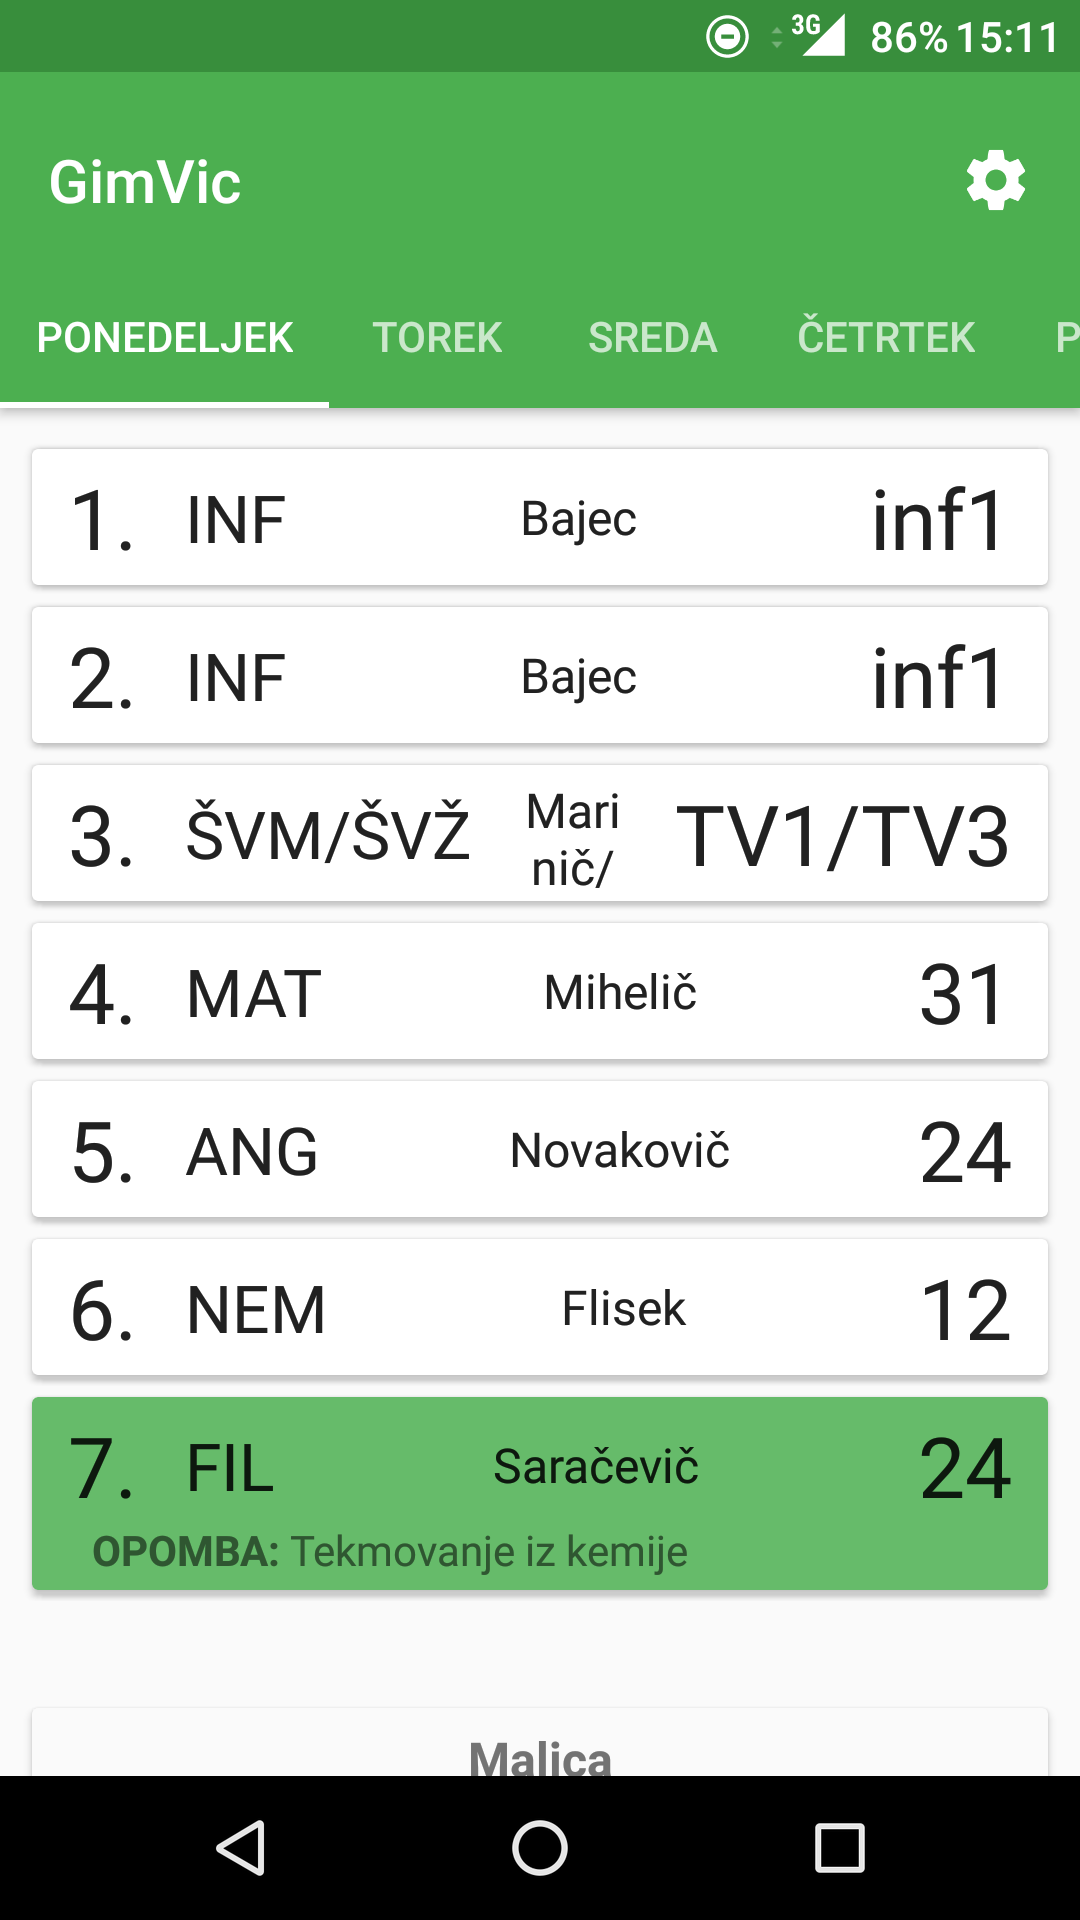
\includegraphics[width=\linewidth]{images/main.png}
  \caption{Glavna stran}\label{fig:main_activity}
\endminipage\hfill
\minipage{0.32\textwidth}
  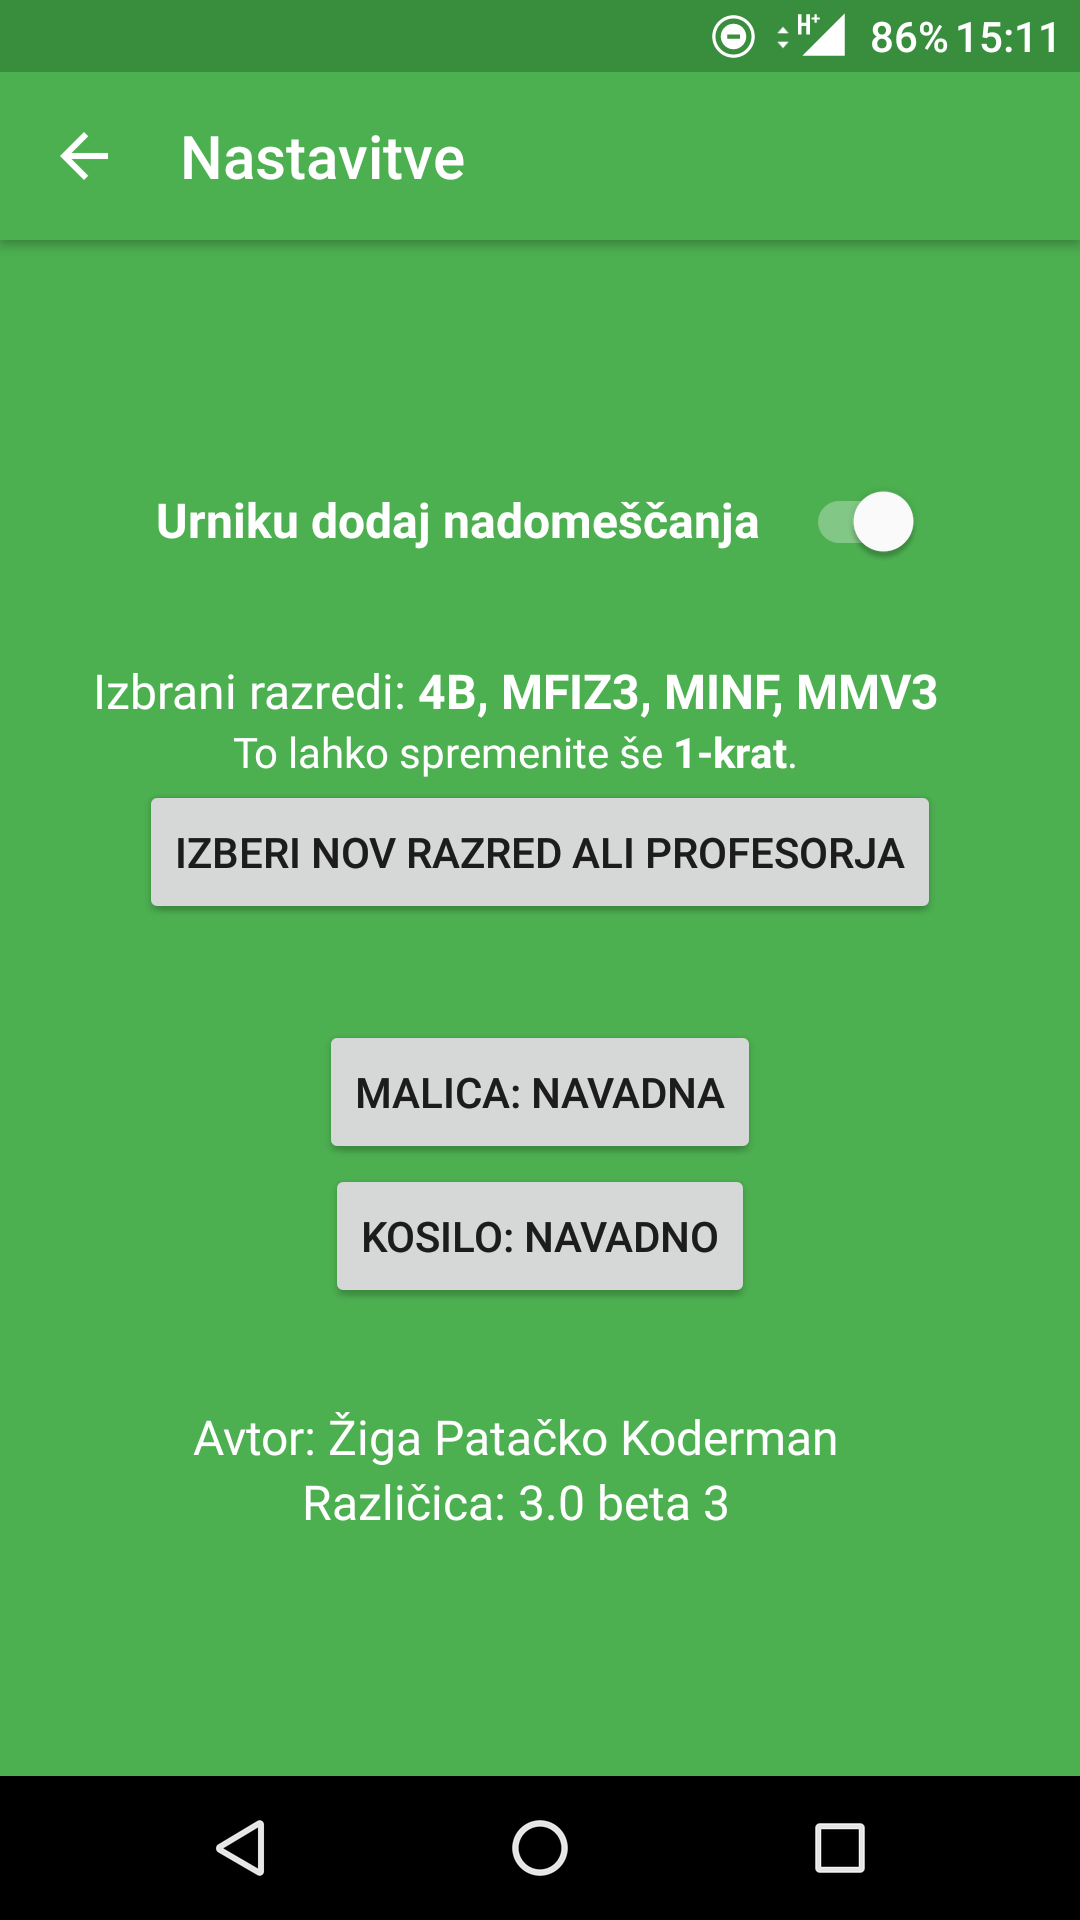
\includegraphics[width=\linewidth]{images/settings.png}
  \caption{Nastavitve}\label{fig:settings_activity}
\endminipage\hfill
\minipage{0.32\textwidth}%
  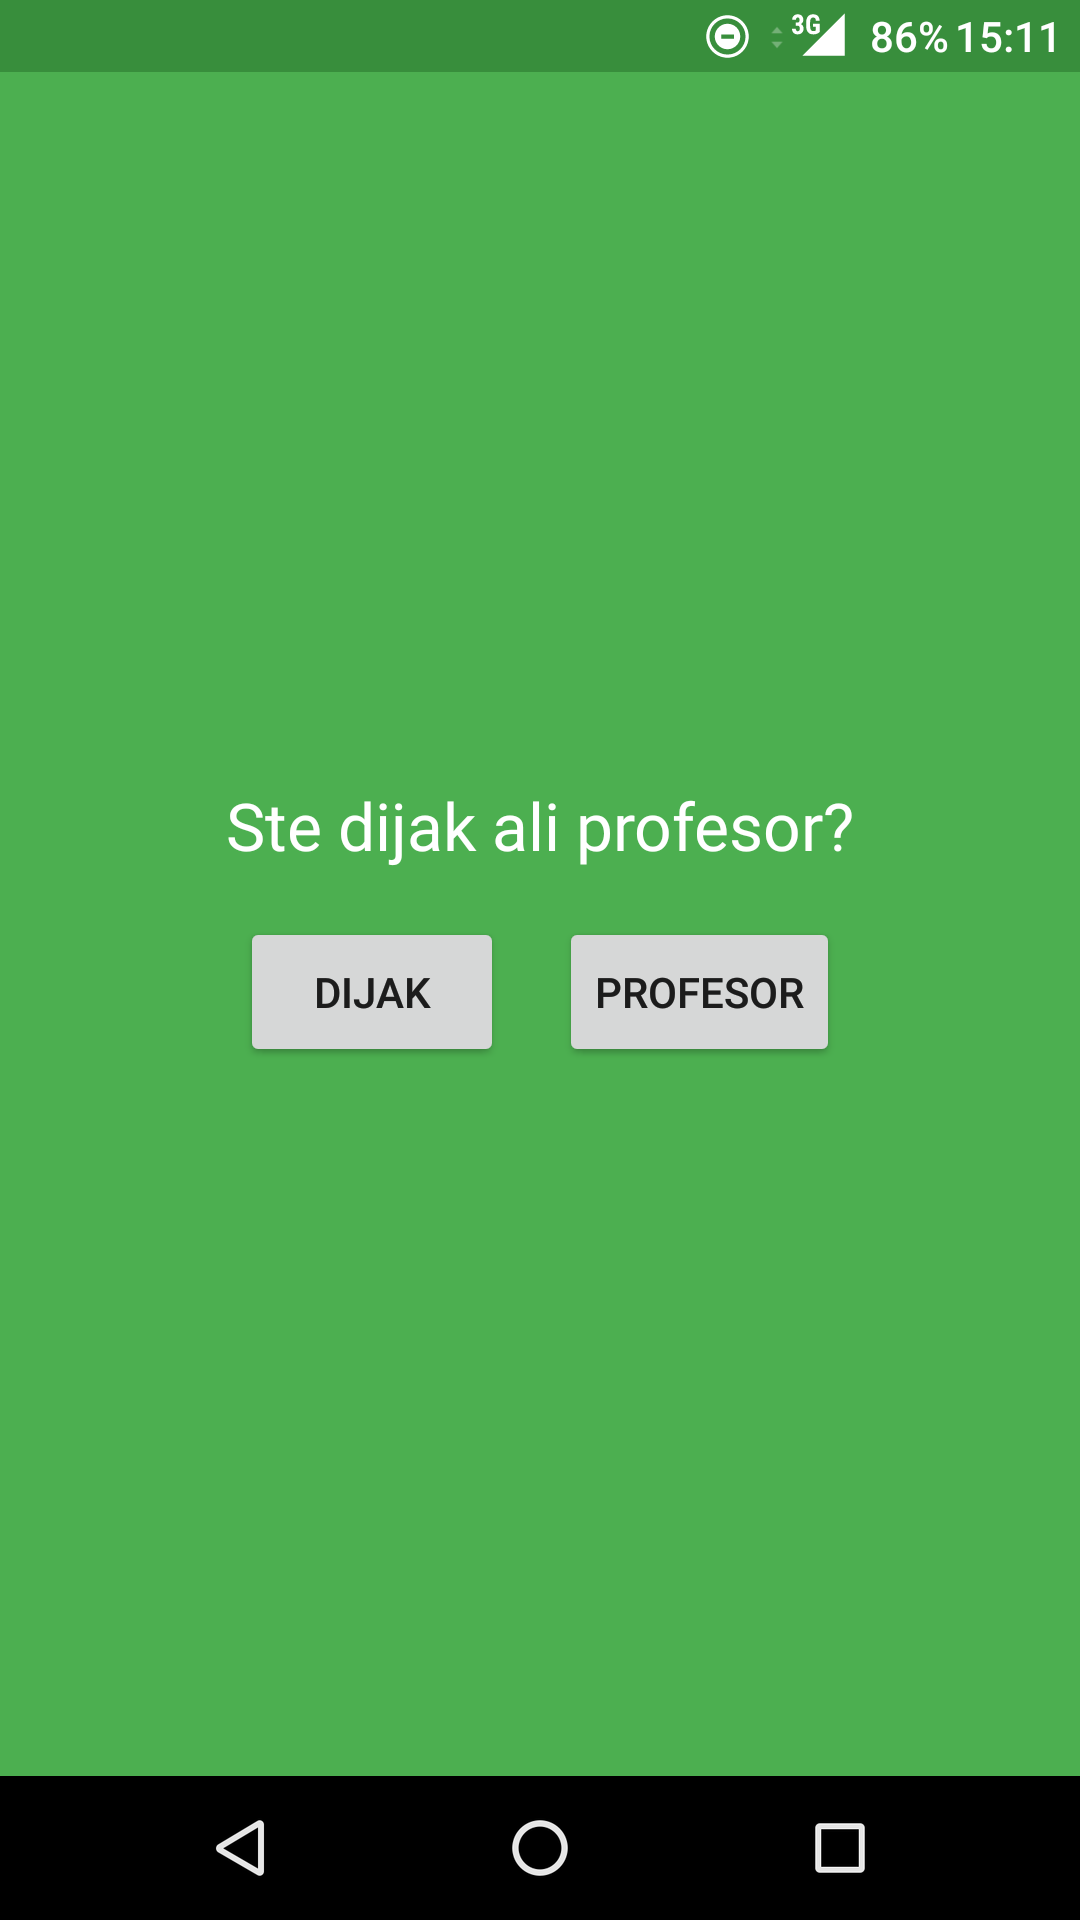
\includegraphics[width=\linewidth]{images/filters.png}
  \caption{Izbira filtrov}\label{fig:filters_activity}
\endminipage
\end{figure}
